We define the \textit{acoustic potential field} $\psi$ as the Fourier transform of the acoustic pressure field, such that, in the \textit{free-field} (i.e., in a region free of sources and scattering bodies), the acoustic potential field satisfies the homogeneous Helmholtz equation,
\begin{equation}\label{eq:02_Acoustical_Theory:Helmholtz_Equation}
\left( \nabla^2 + k^2 \right) \psi(k,\vec{r}) = 0,
\end{equation}
where $\nabla^2$ is the Laplace operator, $k = \omega / c$ is the angular wavenumber, and $c \approx 343$~m/s is the speed of sound.

Depending on our region of interest, we may impose different boundary conditions on the problem in order to ensure that our solution for the acoustic potential field is physically possible.
For example, for an exterior (free-field) region of interest, all sources and obstacles must exist within a spherical region centered on the origin and of some finite radius, $R$.
Consequently, the solution must satisfy the Sommerfeld radiation condition \citep[section 2.1.1]{Zotter2009PhD}, which can be written as
\begin{equation}
\lim_{r\to\infty} \left[ r \left( \frac{\partial}{\partial r} - i k \right) \psi (k,\vec{r}) \right] = 0.
\end{equation}
Although multiple physical interpretations of this condition exist (cf.~\citet[appendix A]{Zotter2009PhD}, \citet[section 4-5]{Pierce1994}), essentially it states that power must only be radiating away from sources located near the origin, rather than arriving from infinity and being destroyed \citep{WikiSommerfeldURL}.
In this case, we must choose singular, radiating basis solutions to the Helmholtz equation, which are given by $h_l(kr) Y_n(\hat{r})$, where $h_l$ is the (outgoing) spherical Hankel function of the first kind and of order $l$, and $Y_n$ is the spherical harmonic for ACN index $n$ \citep[section 6.7]{Williams1999}.
The interested reader is referred to the works of \citet{Zotter2009PhD,Williams1999} for more detailed discussions of such exterior problems.

For an interior region of interest, where all sources exist beyond some finite radius $R$ away from the origin, we require that the solution be finite in magnitude everywhere inside that region, i.e., $|\psi| < \infty,~\forall r < R$.
In this case, we must choose regular (i.e., not singular) basis solutions to the Helmholtz equation, which are given by $j_l(kr) Y_n(\hat{r})$, where $j_l$ is the spherical Bessel function of order $l$ \citep[section 6.8]{Williams1999}.
%These solutions are only valid under free-field conditions, and can be used to describe the acoustic potential in an interior region, that is, for $r < R$, where $R$ is a finite distance .
%So that the region remains source- and obstacle-free, $R$ is typically taken to be the distance of the nearest source or scattering body to the origin.
This spherical interior region where $r < R$ is the so-called \textit{region of validity}, which is illustrated in \figref{fig:02_Acoustical_Theory:Region_of_Validity}.

% Diagram of source/mic positions
\begin{figure}[t]
\centering
  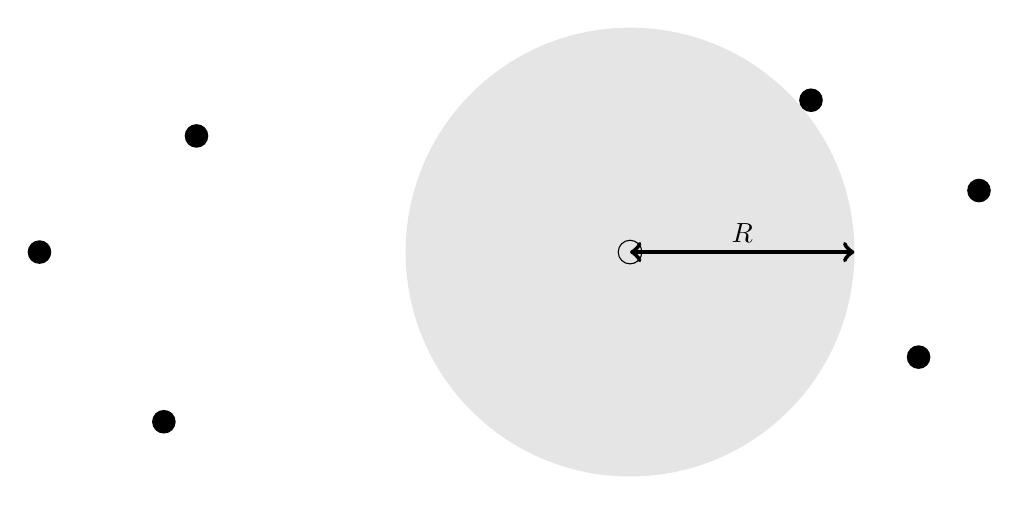
\begin{tikzpicture}[scale=3]
% Parameters
\def\radius{1};
\def\validR{0.95};
\def\sourceR{1-\validR}

\pgfmathsetmacro\evalX{cos(140)*\radius}
\pgfmathsetmacro\evalY{sin(140)*\radius}

\pgfmathsetmacro\sourceXa{cos(-20)*1.3*\radius}
\pgfmathsetmacro\sourceYa{sin(-20)*1.3*\radius}

\pgfmathsetmacro\sourceXb{cos(10)*1.5*\radius}
\pgfmathsetmacro\sourceYb{sin(10)*1.5*\radius}

\pgfmathsetmacro\sourceXc{cos(200)*2.1*\radius}
\pgfmathsetmacro\sourceYc{sin(200)*2.1*\radius}

\pgfmathsetmacro\sourceXd{cos(180)*2.5*\radius}
\pgfmathsetmacro\sourceYd{sin(180)*2.5*\radius}

\pgfmathsetmacro\sourceXe{cos(165)*1.9*\radius}
\pgfmathsetmacro\sourceYe{sin(165)*1.9*\radius}

\pgfmathsetmacro\sourceXf{cos(40)*\radius}
\pgfmathsetmacro\sourceYf{sin(40)*\radius}

\fill [color=black,opacity=0.1] (0,0) circle (\validR*\radius);

%\node at (0,0){$\times$};
\draw [color=black] (0,0) circle (\sourceR*\radius);
\draw[ultra thick,<->] (0,0) -- (\validR*\radius,0);
\node[above] at (0.5*\validR*\radius,0){$R$};

% Source positions
\fill [color=black] (\sourceXa,\sourceYa) circle (\sourceR*\radius);
\fill [color=black] (\sourceXb,\sourceYb) circle (\sourceR*\radius);
\fill [color=black] (\sourceXc,\sourceYc) circle (\sourceR*\radius);
\fill [color=black] (\sourceXd,\sourceYd) circle (\sourceR*\radius);
\fill [color=black] (\sourceXe,\sourceYe) circle (\sourceR*\radius);
\fill [color=black] (\sourceXf,\sourceYf) circle (\sourceR*\radius);
\end{tikzpicture}
  \caption[Diagram of the region of validity for an interior free-field region.]{
  Diagram of the region of validity for a free-field spherical Fourier-Bessel expansion.
  The empty circle indicates the expansion center,
  the filled circles indicate source positions,
  and the shaded disk indicates the region of validity.
  The radius of the region of validity is equal to $R$, the distance of the nearest source from the expansion center.}
  \label{fig:02_Acoustical_Theory:Region_of_Validity}
\end{figure}

Inside this region, any acoustic potential field can be written as an infinite sum of regular solutions, known as a spherical Fourier-Bessel series expansion, given by \citep[chapter 2]{GumerovDuraiswami2005}
\begin{equation}\label{eq:02_Acoustical_Theory:Infinite_Order_Expansion}
\psi(k,\vec{r}) = \sum_{n=0}^{\infty} 4\pi (-i)^l A_n(k) j_l(kr) \frac{Y_n(\hat{r})}{\|Y_n\|^2},
\end{equation}
where $A_n$ are the corresponding (frequency-dependent) expansion coefficients and we have, without loss of generality, factored out $(-i)^l$ to ensure conjugate-symmetry in each $A_n$, making each ambisonics signal (i.e., the inverse Fourier transform of $A_n$) real-valued for a real pressure field.
Note that this expansion need not be taken about the origin, but instead can be taken about any arbitrary expansion center, in which case the region of validity refers to a spherical free-field region centered about that point.
In practice, this expansion is truncated to a finite order $L$ (i.e., $l \in [0,L]$), yielding $N = (L + 1)^2$ terms,
\begin{equation}\label{eq:02_Acoustical_Theory:Finite_Order_Expansion}
\psi(k,\vec{r}) = \sum_{n=0}^{N - 1} 4\pi (-i)^l A_n(k) j_l(kr) \frac{Y_n(\hat{r})}{\|Y_n\|^2}.
\end{equation}